\documentclass[aspectratio=169,11pt]{beamer}

% Shared style (ib-tutorials.sty at the repo root).
\makeatletter\def\input@path{{./}{../}}\makeatother
\usepackage{ib-tutorials}

\usepackage[utf8]{inputenc}
\usepackage{amsmath,amssymb}
\usepackage{booktabs}
\usepackage{array}
\newcolumntype{L}[1]{>{\raggedright\arraybackslash}p{#1}}
\usepackage{graphicx}
\graphicspath{{../pictures/3-ibamr-fundamentals/}{pictures/3-ibamr-fundamentals/}}
\usepackage{xcolor}
\usepackage{listings}
\usepackage{tikz}
\usetikzlibrary{arrows.meta,positioning,shapes.geometric,fit,calc,decorations.pathmorphing}
\usepackage{hyperref}

\newcommand{\sourcecredit}[1]{\vfill\begin{flushright}\tiny\textcolor{DarkGray}{#1}\end{flushright}}

\lstset{
  basicstyle=\ttfamily\scriptsize\color{BlackGray},
  keywordstyle=\color{NavyBlue}\bfseries,
  commentstyle=\color{DarkGray}\itshape,
  stringstyle=\color{OliveGreen},
  showstringspaces=false,
  columns=fullflexible,
  keepspaces=true,
  breaklines=true,
  breakindent=1em,
  frame=single,
  framerule=0.4pt,
  rulecolor=\color{LightGray},
  backgroundcolor=\color{LightGray!30},
  xleftmargin=0.25em,
  xrightmargin=0.25em
}
\lstdefinestyle{shell}{morecomment=[l]{\#}}
\lstdefinestyle{input}{morecomment=[l]{//}}
\lstdefinestyle{matlab}{morecomment=[l]{\%}}
\lstdefinestyle{python}{morecomment=[l]{\#}}
\lstdefinestyle{data}{}
\lstdefinestyle{tiny}{basicstyle=\ttfamily\tiny\color{BlackGray}}
\lstdefinestyle{inputtiny}{morecomment=[l]{//},basicstyle=\ttfamily\tiny\color{BlackGray}}
\lstdefinestyle{matlabtiny}{morecomment=[l]{\%},basicstyle=\ttfamily\tiny\color{BlackGray}}
\lstdefinestyle{pythontiny}{morecomment=[l]{\#},basicstyle=\ttfamily\tiny\color{BlackGray}}
\lstdefinestyle{cpp}{language=C++,morecomment=[l]{//}}
\lstdefinestyle{cpptiny}{language=C++,morecomment=[l]{//},basicstyle=\ttfamily\tiny\color{BlackGray}}
\lstdefinestyle{cmake}{morecomment=[l]{\#}}

\title[Constraint IB]{Constraint IB}
\subtitle{Rigid and prescribed-motion bodies with \code{ConstraintIBMethod}: a kinematics class, the input blocks, the force files, and three upstream examples run}
\author[Miller]{Laura A. Miller}
\institute[UArizona]{Department of Mathematics, University of Arizona}
\date{Using IB Software \textbullet\ Part III \textbullet\ Chapter 14}

\begin{document}

% 1
\begin{frame}[plain]
\maketutorialtitlepanel{%
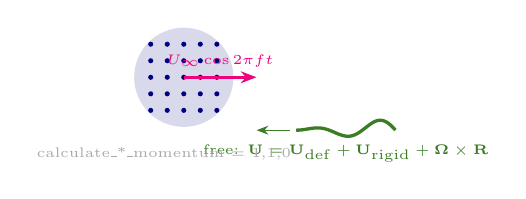
\begin{tikzpicture}[scale=0.84]
  \fill[NavyBlue!15] (1.2,1.4) circle (0.75);
  \foreach \x in {-0.5,-0.25,0,0.25,0.5} \foreach \y in {-0.5,-0.25,0,0.25,0.5} {
    \pgfmathsetmacro{\r}{sqrt(\x*\x+\y*\y)}
    \ifdim \r pt < 0.72pt \fill[NavyBlue] (1.2+\x,1.4+\y) circle (1.1pt); \fi }
  \draw[-{Stealth[length=2mm]},RubineRed,very thick] (1.2,1.4) -- (2.3,1.4);
  \node[font=\tiny,text=RubineRed] at (1.75,1.65) {$U_\infty\cos 2\pi f t$};
  \draw[OliveGreen,very thick] plot[domain=2.9:4.4,samples=40] (\x,{0.6+0.12*(\x-2.9)*sin(deg(6.28*(\x-2.9)))});
  \draw[-{Stealth[length=1.5mm]},OliveGreen] (2.8,0.6) -- (2.3,0.6);
  \node[font=\tiny,text=OliveGreen] at (3.65,0.25) {free: $\mathbf{U} = \mathbf{U}_{\mathrm{def}} + \mathbf{U}_{\mathrm{rigid}} + \boldsymbol{\Omega}\times\mathbf{R}$};
  \node[font=\tiny,text=DarkGray] at (0.9,0.25) {\code{calculate\_*\_momentum = 1,1,0}};
\end{tikzpicture}}
\end{frame}

% 2
\begin{frame}{Learning goals}
\label{fr:goals}
\footnotesize By the end of this chapter you should be able to:
\begin{enumerate}
  \item say what the constraint IB method does that the standard IB method cannot: make a region of fluid move as a rigid body, or as a body whose deformation you prescribe, by correcting the fluid velocity inside it after every solve rather than by springs and beams;
  \item read a ConstraintIB program: \code{ConstraintIBMethod} in place of \code{IBMethod}, a kinematics class that returns the velocity you want, and the two input blocks that tie them to a structure;
  \item write the \code{ConstraintIBKinematics} block for a prescribed body, a free rigid body and a free swimmer, with the keys that exist (the 2020 slides had one that does not);
  \item find the forces, velocities and positions the method writes, and read them with four lines of Python or MATLAB;
  \item build and run the three examples of this chapter (an oscillating cylinder, an impulsively started cylinder, a swimming eel) and say what each shows.
\end{enumerate}
\begin{punchbox}
\footnotesize Chapter 13 gave a point mass; this chapter gives a whole body a rigid motion, prescribed or free. Where the standard IB method asks ``what force does this shape produce?'', the constraint method asks ``what force does it take to make the fluid move like this?'' and applies it.
\end{punchbox}
\end{frame}

% 3
\begin{frame}{How this chapter was checked}
\label{fr:checked}
\begin{itemize}\footnotesize
  \item Every input key, error message and output file is quoted from the IBAMR 0.19.0 sources (\code{ConstraintIBMethod.cpp}, \code{ConstraintIBKinematics.cpp}, the three examples' kinematics classes); the step-by-step account of slide \ref{fr:step} is the method's \code{postprocessSolveFluidEquations}, in order.
  \item The three examples ConstraintIB/01, 02 and 03 are the upstream \code{oscillating\_rigid\_cylinder}, \code{impulsively\_started\_cylinder} and \code{eel2d}, each with its edits listed in its README; they build with 0 warnings against 0.19.0, their MATLAB generators were run under Octave 8.4 and the Python ports write the same files byte for byte (and the same files as shipped upstream), and the figures are from the runs made for this chapter.
  \item The 2020 lecture \emph{Looking at ConstraintIB examples of prescribed and rigid body motion} (IBAMR Lecture 7, 23 slides) and the six ConstraintIB slides of Lecture 6 are quoted in full; where a slide was wrong about the code (a key that does not exist, a file name, what one class does), the slide is quoted and the correction follows it.
\end{itemize}
\begin{punchbox}
\footnotesize Slide numbers refer to this deck; chapter numbers (5, 6, 7, 10, 11, 13, 15, 16, 26) to the other chapters of this series.
\end{punchbox}
\end{frame}

% 4
\begin{frame}{Where to look things up}
\label{fr:lookup}
\small
\begin{itemize}
  \item \al{The method}: \code{include/ibamr/ConstraintIBMethod.h}, \code{src/IB/ConstraintIBMethod.cpp} (the constructor opens the output files; \code{getFromInput} lists the keys; \code{postprocessSolveFluidEquations} is the algorithm).
  \item \al{The kinematics interface}: \code{include/ibamr/ConstraintIBKinematics.h} (four pure virtual functions) and \code{src/IB/ConstraintIBKinematics.cpp} (the \code{StructureParameters} constructor reads the structure block and names the three update methods).
  \item \al{The examples}: \code{examples/ConstraintIB/} in the IBAMR source tree, nine folders (slide \ref{fr:nine}); this series ships three of them as ConstraintIB/01--03 with READMEs and measured results.
  \item \al{The paper}: A. P. S. Bhalla, R. Bale, B. E. Griffith and N. A. Patankar, \emph{A unified mathematical framework and an adaptive numerical method for fluid--structure interaction with rigid, deforming, and elastic bodies}, J.\ Comput.\ Phys.\ 250 (2013) 446--476. Section numbers on slide \ref{fr:nine} are its.
  \item \al{Related tools}: \code{CIBMethod} (chapter 15), \code{IBFEDirectForcingKinematics}, \code{BrinkmanPenalizationRigidBodyDynamics} (slide \ref{fr:tools}).
\end{itemize}
\end{frame}

% 5
\begin{frame}{What the constraint IB method does}
\label{fr:what}
\begin{columns}[T,onlytextwidth]
\begin{column}{0.56\textwidth}
\scriptsize The standard IB method (chapters 5--13) computes a force from the structure's deformation and lets the fluid carry the structure. The constraint method turns this round:
\begin{enumerate}
  \item the fluid is solved everywhere, inside the body too, as if the body were fluid;
  \item the new fluid velocity is interpolated to the body's points, $\mathbf{U}$;
  \item the velocity the body \emph{should} have is assembled,
  \[\mathbf{U}_{\mathrm{new}} = \mathbf{U}_{\mathrm{def}} + \mathbf{U}_{\mathrm{rigid}} - \mathbf{U}_{\mathrm{def,COM}} + \boldsymbol{\Omega}\times\mathbf{R},\]
  from the prescribed deformation velocity and the rigid translation and rotation, which are either prescribed (locked at zero) or computed from the momentum of the fluid in the body;
  \item the correction $(\mathbf{U}_{\mathrm{new}} - \mathbf{U})$ is spread back to the grid, so the fluid in the body region moves as the body does; the force this took, $\rho_s(\mathbf{U}_{\mathrm{new}} - \mathbf{U})/\Delta t$ per point, is the constraint force, and minus its sum is the hydrodynamic force on the body.
\end{enumerate}
\end{column}
\begin{column}{0.42\textwidth}
\scriptsize No springs, no beams, no stiffness to choose and no stiffness-limited time step: the body is rigid to the accuracy of the interpolation and the fluid solver's CFL limit is the only one. The price: the body is a region of fluid of the fluid's density ($\rho_{\mathrm{solid}} = \rho_{\mathrm{fluid}}$ is assumed; a heavier body gets a body force instead, slide \ref{fr:free}), and a deforming body must have its deformation prescribed, not computed from elasticity (that is IBFE's job, Part IV).
\end{column}
\end{columns}
\end{frame}

% 6
\begin{frame}{The 2020 lecture's framing}
\label{fr:lecture}
\footnotesize \al{IBAMR Lecture 7 (2020), slide 2, repeating Lecture 6's slide 18:} ``Constraint IB Examples. \emph{A unified mathematical framework and an adaptive numerical method for fluid--structure interaction with rigid, deforming, and elastic bodies}, Amneet Pal Singh Bhalla, Rahul Bale, Boyce E. Griffith, Neelesh A. Patankar. This paper is on the google drive. Note that it is the first paper for rigid body simulations. Nearly all of the examples considered in this paper appear in these Constraint IB examples. Some examples are also similar to the CIB ones. Some of the examples generate HUGE numbers of files.''
\vspace{1mm}

\footnotesize Slide 3 was a screenshot of the folder \code{examples/ConstraintIB} with its nine sub-folders (slide \ref{fr:nine}). Lecture 6, which toured IBAMR's example tree, had introduced four of them in one slide each; Lecture 7 then opened three of them file by file: the oscillating cylinder (prescribed motion), the impulsively started cylinder (rigid-body motion) and the 2D eel (prescribed deformation, free swimming). This chapter follows that order and runs all three.
\begin{punchbox}
\footnotesize ``HUGE numbers of files'': the upstream inputs dump visualization every 40 steps and, in the eel's case, restart files every 150 steps, for runs of 100,000 steps and more. The examples of this series shorten the runs and the dump intervals (each README's ``History'').
\end{punchbox}
\end{frame}

% 7
\begin{frame}{The nine upstream examples (1): prescribed motion}
\label{fr:nine}
\scriptsize
\setlength{\tabcolsep}{3pt}
\begin{tabular}{@{}L{0.29\textwidth}L{0.2\textwidth}lL{0.38\textwidth}@{}}
\toprule
folder & body and motion & paper & the lecture (2020) \\
\midrule
\code{stokes\_first\_problem} & a plate started impulsively & 7.1.1 & ``an infinitely long horizontal plate is impulsively started with a velocity $U_0$ in the $x$ direction''\\
\code{moving\_plate} & a finite plate dragged across the fluid & 7.1.2 & ``a finite plate of height $b$ in an infinite quiescent flow that is dragged perpendicular to itself with a constant velocity $U_0$''\\
\code{oscillating\_rigid\_cylinder} & a disc oscillating; \al{ConstraintIB/01} & 7.1.4 & ``contributions to the drag forces come from both inertial and constraint forces''\\
\code{flow\_past\_cylinder} & a disc towed at constant speed & -- & (not shown; the same files as 01 with \code{prescribed\_trans\_velocity})\\
\bottomrule
\end{tabular}
\vspace{1mm}

\scriptsize All four lock every rigid degree of freedom (\code{calculate\_*\_momentum = 0,0,0}): the body moves as its kinematics class says and the force files are the result. Lecture 6 introduced the plate, the Stokes plate and the oscillating cylinder in one slide each (slides 20, 22, 23), quoting the paper's section for each; Lecture 7 opened the oscillating cylinder file by file (slides 4--12). The paper's quotes above are the lecture's; its slide on the impulsively started cylinder read ``$D$ ¼ 1 m'' and ``16 mat time'' where the PDF's glyphs had been copied (it means $D = 1$ m and ``16 m at time'').
\end{frame}

% 7b
\begin{frame}{The nine upstream examples (2): free motion}
\label{fr:nine2}
\scriptsize
\setlength{\tabcolsep}{3pt}
\begin{tabular}{@{}L{0.29\textwidth}L{0.2\textwidth}lL{0.38\textwidth}@{}}
\toprule
folder & body and motion & paper & the lecture (2020) \\
\midrule
\code{impulsively\_started\_cylinder} & a disc given an impulse; free rigid body; \al{ConstraintIB/02} & 7.2.2 & ``to demonstrate the momentum-conservation properties of our method \ldots an impulse of the form $I(t) = 400\exp(-400t)$ N/m$^3$ is applied in the $x$ direction within the body''\\
\code{falling\_sphere} & a sphere sinking under gravity, 3D; free & -- & ``we impose a gravitational body force that is present only in the solid region''\\
\code{eel2d} & a deforming eel, free swimming; \al{ConstraintIB/03} & 7.3 & ``the body deforms in a prescribed manner but is propelled through the water due to rigid body motion''\\
\code{eel3d}, \code{knifefish} & the same in 3D; a knifefish with a ribbon fin & 7.3 & ``It is worth running the 3D eel and knifefish as well.''\\
\bottomrule
\end{tabular}
\vspace{1mm}

\scriptsize These unlock translation and rotation (\code{1,1,0} and \code{0,0,1} in 2D; all six in 3D): the body takes the momentum of the fluid in it. Lecture 6, slide 24: ``Other examples include free swimming cases of eel swimming in 2D and 3D as well as a 3D knifefish. I have run the 2D eel, but the download is taking too long to show today. It is worth running the 3D eel and knifefish as well. There is also a falling sphere example of rigid body motion in 3D. `We validate our algorithm for a freely moving body by considering the problem of a sedimenting sphere. To treat this problem with our present formulation and implementation, which assume that the mass density of the fluid--structure system is uniform, we impose a gravitational body force that is present only in the solid region $\Omega_c$ of the physical domain $\Omega$.'\,'' Lecture 7 opened the impulsively started cylinder (slides 13--18) and the eel (19--23).
\end{frame}

% 8
\begin{frame}[fragile]{A ConstraintIB program: the three pieces}
\label{fr:program}
\vspace{-3pt}
\begin{columns}[T,onlytextwidth]
\begin{column}{0.52\textwidth}
\begin{lstlisting}[style=cpptiny]
// main.cpp (ConstraintIB/01): 1. the method replaces IBMethod
#include <ibamr/ConstraintIBMethod.h>
const int num_structures =
    input_db->getIntegerWithDefault("num_structures", 1);
Pointer<ConstraintIBMethod> ib_method_ops = new ConstraintIBMethod(
    "ConstraintIBMethod",
    app_initializer->getComponentDatabase("ConstraintIBMethod"),
    num_structures);
Pointer<IBHierarchyIntegrator> time_integrator =
    new IBExplicitHierarchyIntegrator("IBHierarchyIntegrator",
        app_initializer->getComponentDatabase("IBHierarchyIntegrator"),
        ib_method_ops, navier_stokes_integrator);
time_integrator->initializePatchHierarchy(
    patch_hierarchy, gridding_algorithm);
// 2. one kinematics object per structure, from its sub-block of the input
vector<Pointer<ConstraintIBKinematics>> ibkinematics_ops_vec;
Pointer<ConstraintIBKinematics> ib_kinematics_op;
ib_kinematics_op = new OscillatingCylinderKinematics(
    "Cylinder",
    app_initializer->getComponentDatabase("ConstraintIBKinematics")
                   ->getDatabase("Cylinder"),
    ib_method_ops->getLDataManager(), patch_hierarchy);
ibkinematics_ops_vec.push_back(ib_kinematics_op);
// 3. register them, then build the method's operators and data
ib_method_ops->registerConstraintIBKinematics(
    ibkinematics_ops_vec);
ib_method_ops->initializeHierarchyOperatorsandData();
\end{lstlisting}
\end{column}
\begin{column}{0.46\textwidth}
\scriptsize The rest of \code{main.cpp} is the program of IB/01 (chapter 6): the Navier--Stokes integrator, the grid, \code{IBStandardInitializer} reading the \code{.vertex} file, the boundary conditions, the viz writers and the time loop are unchanged. Three things are new:
\begin{enumerate}
  \item \code{ConstraintIBMethod} takes the place of \code{IBMethod}, with the number of structures it will constrain;
  \item after the hierarchy exists, one \code{ConstraintIBKinematics} object is made per structure, from the sub-block of \code{ConstraintIBKinematics} that bears the structure's name;
  \item \code{initializeHierarchyOperatorsandData()} is called once the objects are registered.
\end{enumerate}
\end{column}
\end{columns}
\end{frame}

% 8b
\begin{frame}[fragile]{A ConstraintIB program (2): the lecture's slides, and the other two examples' versions}
\label{fr:program2}
\begin{columns}[T,onlytextwidth]
\begin{column}{0.5\textwidth}
\scriptsize The lecture's slides 11, 12 and 18 (``Example.cpp'', ``Example.cpp continued'', ``Other relevant parts of example.cpp'') showed exactly the lines of slide \ref{fr:program}: the \code{\#include}, the \code{new ConstraintIBMethod(...)} with its three arguments, and the block that creates, registers and initializes the kinematics objects, for the oscillating cylinder (slide 12) and for the impulsively started one (slide 18).
\vspace{1mm}

\scriptsize Three things to notice:
\begin{itemize}
  \item \code{num\_structures}: the input may set it (02 and 03 do, \code{num\_structures = 1}); the number of kinematics objects pushed into the vector must match it;
  \item the first argument of the kinematics constructor is an object name for restarts; the second is the \emph{sub-block} of \code{ConstraintIBKinematics} bearing the structure's block name, so a renamed block needs a renamed \code{getDatabase};
  \item \code{patch\_hierarchy} is passed so that a class can look at the grid (the eel's does, to place its points one cell apart).
\end{itemize}
\end{column}
\begin{column}{0.48\textwidth}
\begin{lstlisting}[style=cpptiny]
// ConstraintIB/02: a rigid body with no deformation
ib_kinematics_op = new RigidBodyKinematics(
    "CYLINDER_2D",
    app_initializer->getComponentDatabase("ConstraintIBKinematics")
                   ->getDatabase("Cylinder2d"),
    ib_method_ops->getLDataManager(), patch_hierarchy);
// ConstraintIB/03: the eel, plus the control-volume force evaluator
ib_kinematics_op = new IBEELKinematics(
    "eel2d",
    app_initializer->getComponentDatabase("ConstraintIBKinematics")
                   ->getDatabase("eel2d"),
    ib_method_ops->getLDataManager(), patch_hierarchy);
Pointer<IBHydrodynamicForceEvaluator> hydro_force =
    new IBHydrodynamicForceEvaluator("IBHydrodynamicForce",
        rho_fluid, mu_fluid, start_time, true);
hydro_force->registerStructure(box_X_lower, box_X_upper,
    patch_hierarchy, box_init_vel, 0);
\end{lstlisting}
\scriptsize The upstream \code{moving\_plate} goes one step further: its \code{RigidBodyKinematics} object gets a callback, \code{registerRigidBodyKinematics(\&COMTransVelocity, nullptr)}, a C function returning the plate's velocity, instead of input expressions.
\end{column}
\end{columns}
\end{frame}

% 9
\begin{frame}[fragile]{The kinematics class: four functions, and the oscillating cylinder's}
\label{fr:kin}
\begin{columns}[T,onlytextwidth]
\begin{column}{0.5\textwidth}
\scriptsize \code{ConstraintIBKinematics} is abstract; a subclass must provide
\begin{lstlisting}[style=cpptiny]
virtual void setKinematicsVelocity(const double time,
    const std::vector<double>& incremented_angle_from_reference_axis,
    const std::vector<double>& center_of_mass,
    const std::vector<double>& tagged_pt_position) = 0;
virtual const std::vector<std::vector<double>>& getKinematicsVelocity(const int level) const = 0;
virtual void setShape(const double time,
    const std::vector<double>& incremented_angle_from_reference_axis) = 0;
virtual const std::vector<std::vector<double>>& getShape(const int level) const = 0;
\end{lstlisting}
\scriptsize The method calls \code{setKinematicsVelocity} and then \code{setShape} once per step with the time, the body's accumulated rotation, its centre of mass and the position of the tagged point; it then reads back the velocity, \code{[component][point]} per level, and the shape (used only in the \code{CONSTRAINT\_POSITION} modes). The base class's \code{StructureParameters} tells the subclass its index range, levels and which rigid components are free.
\end{column}
\begin{column}{0.48\textwidth}
\begin{lstlisting}[style=cpptiny]
// OscillatingCylinderKinematics.cpp (upstream, unchanged)
if (input_db->keyExists("frequency")) d_freq = input_db->getDouble("frequency");
else TBOX_ERROR("... frequency of cylinder does not exist in the InputDatabase ...");
...
void OscillatingCylinderKinematics::setOscillatingCylinderSpecificVelocity(const double time)
{
    ...
    for (int k = 0; k < number_lag_points; ++k)
    {
        d_current_kinematics_vel[0][0][k] = d_prescribed_trans_vel + d_Uinf * std::cos(2 * M_PI * d_freq * time);
    }
}
\end{lstlisting}
\scriptsize ``\code{d\_current\_kinematics\_vel[0][0][k]} -- this refers to level 0 (should usually be 0), the component of velocity (0 is x), and k is the vertex number.'' (2020, slide 6). The first index is the level \emph{offset} from the structure's coarsest level, which is why it is 0 for a structure on one level; the class refuses a structure on more than one (``Total levels > 1'').
\end{column}
\end{columns}
\end{frame}

% 10
\begin{frame}[fragile]{The \code{ConstraintIBKinematics} block: the keys that exist}
\label{fr:keys}
\begin{columns}[T,onlytextwidth]
\begin{column}{0.46\textwidth}
\begin{lstlisting}[style=inputtiny]
// input2d (ConstraintIB/01)
ConstraintIBKinematics {
     Cylinder {
     structure_names                  = "cylinder2d"
     structure_levels                 = MAX_LEVELS - 1
     calculate_translational_momentum = 0,0,0
     calculate_rotational_momentum    = 0,0,0
     lag_position_update_method       = "CONSTRAINT_VELOCITY"
     tagged_pt_identifier             = MAX_LEVELS - 1, 0  // level, relative idx of lag point
     // Cylinder oscillates with U_infinity * cos(2*pi*freq*t)
     frequency                        = 0.2
     U_infinity                       = 1.0
     // Additional prescribed velocity
     prescribed_trans_velocity        = 0.0
    }
}
\end{lstlisting}
\scriptsize The sub-block's name (\code{Cylinder}) is what \code{main.cpp} asks for; the structure's name (\code{cylinder2d}) is the \code{.vertex} file's and must also be in \code{IBStandardInitializer}'s list, on the same level.
\end{column}
\begin{column}{0.52\textwidth}
\scriptsize Read by the base class (\code{StructureParameters}), all required:
\begin{itemize}
  \item \code{structure\_names}, \code{structure\_levels}: the structure(s) this object drives and their levels; a name not found gives ``\code{Structure X does not exist on level N}'';
  \item \code{calculate\_translational\_momentum}, \code{calculate\_rotational\_momentum}: three integers each, 1 for every rigid component that is \emph{free} (computed from the fluid's momentum), 0 for locked; the third is the $z$ direction, which 2D does not have;
  \item \code{lag\_position\_update\_method}: \code{CONSTRAINT\_VELOCITY} (positions follow the corrected velocity), \code{CONSTRAINT\_POSITION} (positions set from the shape the class returns, plus the rigid motion) or \code{CONSTRAINT\_EXPT\_POSITION}; anything else stops with a message naming the three;
  \item \code{tagged\_pt\_identifier}: a level and a point index relative to the structure's first; the point's position is handed to \code{setKinematicsVelocity} every step (the eel uses it to steer).
\end{itemize}
The subclass's own keys: next slide.
\end{column}
\end{columns}
\end{frame}

% 10b
\begin{frame}{The \code{ConstraintIBKinematics} block (2): the subclass's own keys}
\label{fr:keys2}
\vspace{-3pt}
\scriptsize Each kinematics class reads what it needs from the same sub-block, after the base class has read the six keys of slide \ref{fr:keys}. The three classes of this chapter:
\setlength{\tabcolsep}{3pt}
\begin{tabular}{@{}L{0.3\textwidth}L{0.36\textwidth}L{0.29\textwidth}@{}}
\toprule
class (example) & keys & if missing \\
\midrule
\code{OscillatingCylinderKinematics} (01) & \code{frequency}, \code{U\_infinity}; \code{prescribed\_trans\_velocity} (a steady drift added to the oscillation) & the first two: \code{TBOX\_ERROR}, the run stops; the third defaults to 0 \\
\code{RigidBodyKinematics} (02) & \code{kinematics\_velocity\_function\_0}, \code{\_1}: muParser expressions of \code{t} and of the centre of mass \code{X0}, \code{X1}, the velocity every point gets besides the rigid motion & a \code{TBOX\_WARNING} per missing one and \code{"0.0"} \\
\code{IBEELKinematics} (03) & \code{body\_shape\_equation}; \code{deformation\_velocity\_function\_0}, \code{\_1} (expressions of \code{X\_0}, \code{T} and the normal \code{N\_0}, \code{N\_1}); \code{initial\_angle\_body\_axis\_0}; \code{body\_is\_maneuvering}, \code{maneuvering\_axis\_equation}, \code{maneuvering\_axis\_is\_changing\_shape}; \code{food\_location\_in\_domain\_0}, \code{\_1} & the shape equation and the food location are required; the velocity functions warn and default to \code{"0.0"}; the angle and the manoeuvring switches default to 0 and \code{FALSE} (the axis equation is read only when manoeuvring) \\
\bottomrule
\end{tabular}

\scriptsize The parser variables: \code{t}/\code{T} for time, \code{X0}/\code{X\_0}/\code{x0}/\code{x\_0} for the first coordinate (the centre of mass in 02, the body coordinate in 03), and in the eel \code{N0}/\code{N\_0} for the body normal; \code{pi}, \code{Pi}, \code{PI} are defined. These are the classes' conventions, not the method's: a class of your own reads whatever keys it declares.
\end{frame}

% 11
\begin{frame}[fragile]{The \code{ConstraintIBMethod} block and \code{PrintOutput}}
\label{fr:method}
\vspace{-3pt}
\begin{columns}[T,onlytextwidth]
\begin{column}{0.46\textwidth}
\begin{lstlisting}[style=inputtiny]
// input2d (ConstraintIB/01)
ConstraintIBMethod {
   delta_fcn                = DELTA_FUNCTION
   enable_logging           = ENABLE_LOGGING
   num_INS_cycles           = NUM_CYCLES
   needs_divfree_projection = FALSE
   rho_solid                = RHO
   PrintOutput {
   print_output          = TRUE               //default false
   output_interval       = 1                  //default 1
   output_drag           = TRUE               //default false
   output_power          = FALSE              //default false
   output_rig_transvel   = TRUE               //default false
   output_rig_rotvel     = TRUE               //default false
   output_com_coords     = TRUE               //default false
   output_moment_inertia = TRUE               //default false
   output_dirname        = "./Dump--Cylinder"  // default ./ConstraintIBMethodDump
   base_filename         = "Cylinder"      //default  "ImmersedStructure"
  }
}
\end{lstlisting}
\end{column}
\begin{column}{0.52\textwidth}
\scriptsize \code{getFromInput} reads, besides \code{IBMethod}'s own keys: \code{needs\_divfree\_projection} (default false: project the spread correction to be divergence-free; 02 sets it), \code{rho\_solid} (one value per structure; equal to the fluid's in every example), \code{rho\_fluid}, \code{calculate\_structure\_linear\_mom} and \code{calculate\_structure\_rotational\_mom} (the body's own momenta, written to the log). The \code{PrintOutput} sub-block: \code{print\_output}, \code{output\_interval}, \code{output\_drag}, \code{output\_torque}, \code{output\_power}, \code{output\_rig\_transvel}, \code{output\_rig\_rotvel}, \code{output\_com\_coords}, \code{output\_moment\_inertia}, \code{output\_eulerian\_mom}, \code{output\_dirname}, \code{base\_filename}, and \code{restart\_output\_dump\_dir} for restarted runs. That is the whole list.

\scriptsize The lecture's slide 10 showed a different block: next slide.
\end{column}
\end{columns}
\end{frame}

% 11b
\begin{frame}[fragile]{The lecture's \code{PrintOutput} block, and why nothing read it}
\label{fr:method2}
\begin{columns}[T,onlytextwidth]
\begin{column}{0.5\textwidth}
\begin{lstlisting}[style=inputtiny]
// IBAMR Lecture 7 (2020), slide 10, "Input2d - print output", as shown
PrintOutput {

    print_output                = TRUE    //default false, if false nothing will be printed.
    output_interval             = 1       //default 1
    output_drag_kinetic_energy  = TRUE    //default false, if false it will not be computed.
    output_power                = FALSE    //default false, if false it will not be computed.
    output_rig_transvel         = FALSE    //default false
    output_rig_rotvel           = FALSE    //default false
    output_com_coords           = FALSE    //default false
    output_moment_inertia       = FALSE   //default false
    output_dirname              = "./cylinder_dump"
    base_filename               = "cylinder2d"
}
\end{lstlisting}
\end{column}
\begin{column}{0.48\textwidth}
\scriptsize Two things are wrong with this block, and neither showed up in 2020:
\begin{itemize}
  \item \code{output\_drag\_kinetic\_energy} is not a key: \code{getFromInput} asks for \code{output\_drag} (slide \ref{fr:method}) and never looks for this one. An unknown key in an IBAMR input block is ignored without a word.
  \item the block sat at the \emph{top level} of the upstream input, after \code{ConstraintIBKinematics}, not inside \code{ConstraintIBMethod}. The method reads only its own sub-block, so this one was never read at all: no \code{cylinder\_dump} folder, no \code{cylinder2d\_*} files.
\end{itemize}
\scriptsize The run therefore printed what the \emph{inner} block (slide \ref{fr:method}) asked for, into \code{Dump--Cylinder}, drag included. The upstream input still carries both blocks; ConstraintIB/01 removes the stray one and documents the real one. The general lesson is chapter 16's: a misplaced or misspelt key fails silently, so check the output folder, not the input, for what you asked for.
\end{column}
\end{columns}
\end{frame}

% 12
\begin{frame}{What the method writes: the files and their columns}
\label{fr:files}
\scriptsize Processor 0 opens one file per quantity in \code{output\_dirname} at start-up, named \code{<base\_filename>\_<quantity>\_struct\_no\_<k>} for structure $k$, and appends one tab-separated line every \code{output\_interval} steps, time first (times $\rho_{\mathrm{solid}}/\Delta t$ where a force is meant):
\begin{center}
\begin{tabular}{@{}lL{0.6\textwidth}@{}}
\toprule
file & columns after the time\\
\midrule
\code{\_Drag\_force\_struct\_no\_k} & inertial force $x, y, z$ (from the change of the points' velocity over the step); constraint force $x, y, z$ (from the correction): their sum is the force on the fluid\\
\code{\_Torque\_struct\_no\_k} & torque, the same two parts\\
\code{\_Power\_spent\_struct\_no\_k} & power of the constraint force\\
\code{\_Trans\_vel\_struct\_no\_k} & rigid translational velocity $x, y, z$; velocity of the centre of mass due to the deformation $x, y, z$\\
\code{\_Rot\_vel\_struct\_no\_k} & rigid angular velocity $x, y, z$; angular velocity of the deformation $x, y, z$\\
\code{\_COM\_coordinates\_struct\_no\_k} & centre of mass $x, y, z$\\
\code{\_MOI\_struct\_no\_k} & the $3\times3$ moment-of-inertia tensor, row by row\\
\code{\_EULERIAN\_MOMENTUM.TXT} & total momentum of the fluid in the box $x, y, z$ (one file for all structures)\\
\bottomrule
\end{tabular}
\end{center}
\scriptsize Three columns in 2D as in 3D: the third is zero. The folder is created by the method; a file whose quantity is switched off is created empty. \code{np.loadtxt(name)} or MATLAB's \code{load(name)} reads any of them (slide \ref{fr:read}); chapter 11's readers are not needed, since these are plain numbers.
\end{frame}

% 13
\begin{frame}{What happens each step, from the source}
\label{fr:step}
\footnotesize \code{ConstraintIBMethod::postprocessSolveFluidEquations}, after the fluid solver has produced the new velocity:
\begin{enumerate}\scriptsize
  \item \code{calculateCOMandMOIOfStructures}: the centre of mass and moment of inertia of each structure from its points (written if asked);
  \item \code{interpolateFluidSolveVelocity}: the new fluid velocity interpolated to the points, $\mathbf{U}$;
  \item \code{calculateKinematicsVelocity}: the accumulated angle is advanced, $\theta_{n} = \theta_{n-1} + \omega_{n-1}\Delta t$; the kinematics object's \code{setKinematicsVelocity} and \code{setShape} are called; for a self-translating body the momentum of the deformation velocity is computed, to be subtracted;
  \item \code{calculateRigidTranslationalMomentum}, \code{calculateRigidRotationalMomentum}: for every free component, the rigid velocity is the \emph{mean} of $\mathbf{U}$ over the structure's points (the momentum of the fluid in the body, per unit mass), and the angular velocity its moment about the centre of mass divided by the moment of inertia; locked components are zero;
  \item \code{correctVelocityOnLagrangianMesh}: $\mathbf{U}_{\mathrm{new}} = \mathbf{U}_{\mathrm{def}} + \mathbf{U}_{\mathrm{rigid}} - \mathbf{U}_{\mathrm{def,COM}} + \boldsymbol{\Omega}\times\mathbf{R}$ at every point, and the correction $(\mathbf{U}_{\mathrm{new}} - \mathbf{U})\times$ the volume per point;
  \item \code{spreadCorrectedLagrangianVelocity}: the correction is spread to the grid, so the fluid in the body region now moves with the body; \code{applyProjection} if \code{needs\_divfree\_projection};
  \item \code{calculateDrag}, \code{Torque}, \code{EulerianMomentum}, \code{Power}, \code{StructureMomentum}: the outputs of slide \ref{fr:files};
  \item then the IB integrator moves the points with the corrected velocity (\code{CONSTRAINT\_VELOCITY}), or places them from the shape plus the rigid motion (\code{CONSTRAINT\_POSITION}).
\end{enumerate}
\scriptsize The ``inertial force'' of the drag file is $\rho_s(\mathbf{U}_{\mathrm{new}} - \mathbf{U}_{\mathrm{current}})\,V/\Delta t$ summed over the points, the ``constraint force'' $\rho_s\,\mathbf{U}_{\mathrm{corr}}/\Delta t$ summed; the paper's section 7.1.4 is about why both are needed for a body whose velocity changes.
\end{frame}

% 14
\begin{frame}{Prescribed, free, and in between: the flags}
\label{fr:free}
\begin{columns}[T,onlytextwidth]
\begin{column}{0.5\textwidth}
\footnotesize
\begin{itemize}
  \item \al{All locked} (\code{0,0,0} and \code{0,0,0}): the body moves exactly as the kinematics object says, and the force files tell you what that cost. The plate, the Stokes plate, the oscillating and the towed cylinder.
  \item \al{Free rigid body} (\code{1,1,0} and \code{0,0,1} in 2D) with zero kinematics velocity: the body moves with the momentum of the fluid in it, which the fluid got from a body force (the impulse of 02, gravity in the solid region for the falling sphere) or from the flow around it.
  \item \al{Free swimmer}: the same flags with a deformation velocity and shape: the eel, the 3D eel, the knifefish. The deformation's own momentum is removed, so a swimmer moves only by what it does to the fluid.
  \item \al{Partly free}: any mix, e.g.\ \code{1,0,0}: a body on rails.
\end{itemize}
\end{column}
\begin{column}{0.48\textwidth}
\footnotesize \al{Density.} The formulation ``assumes that the mass density of the fluid--structure system is uniform'' (the paper, quoted by Lecture 6 for the falling sphere). \code{rho\_solid} scales the forces; it does not give the body extra inertia. A heavier body in this method gets a body force equal to its excess weight, applied only inside the body: ``we impose a gravitational body force that is present only in the solid region''. Chapter 13's penalty method and IBFE with a density (Part IV) are the ways to a body that is really heavier.
\vspace{1mm}

\footnotesize \al{Added mass} comes for free: the fluid inside the body is part of the fluid, so an accelerating body drags its own volume of fluid along and the impulse of 02 is shared (slide \ref{fr:ex02b}).
\end{column}
\end{columns}
\end{frame}

% 15
\begin{frame}[fragile]{ConstraintIB/01: the oscillating cylinder}
\label{fr:ex01}
\begin{columns}[T,onlytextwidth]
\begin{column}{0.5\textwidth}
\scriptsize ``This is a prescribed motion example from 7.1.4. `In cases in which the body has a nonconstant specified velocity, contributions to the drag forces come from both inertial and constraint forces. In this example, we consider a rigid circular cylinder oscillating about a mean position in a quiescent fluid.'\,'' (2020, slide 4)
\begin{itemize}\scriptsize
  \item a disc of diameter $1$ m, $12{,}851$ points one finest cell apart (\code{Cylinder2d.m}: ``The cylinder is filled in and ds=dx''; the lecture's ``2dcylinder.vertex'' is \code{cylinder2d.vertex}), velocity $U_\infty\cos 2\pi f t$ with $f = 0.2$ Hz and $U_\infty = 1$ m/s;
  \item $\mathrm{Re} = 100$ (\code{MU = 2.0*R/Re}), $\mathrm{KC} = U_\infty/fD = 5$: it travels $1.6$ diameters each half period and meets its own wake;
  \item a $32\times16$ m periodic box, $64\times32$ cells on the coarsest level and four levels refined by 4, so the finest cells are $1/128$ m ($128$ across the disc); \code{DT\_MAX = 0.0015};
  \item ``Be sure to include the header file when running simulations.'' (slide 6): \code{OscillatingCylinderKinematics.h}, and the \code{.cpp} in the CMake list.
\end{itemize}
\end{column}
\begin{column}{0.48\textwidth}
\begin{lstlisting}[style=inputtiny]
// input2d: the lines slide 8 showed, as shipped (N is cells per 8 m)
R  = 0.5
Re = 100.0
MU = 2.0*R/Re
RHO = 1.0
MAX_LEVELS = 4        // maximum number of levels in locally refined grid
REF_RATIO  = 4        // refinement ratio between levels
REF_RATIO_FINEST = 4  // refinement ratio for the finest level.
N = 16                // grid cells per 8 m on the coarsest level: ...
NFINEST = (REF_RATIO^(MAX_LEVELS - 1))*N
L = 16
\end{lstlisting}
\scriptsize Slide 8 called \code{N} ``coarsest grid spacing'': it is a cell \emph{count}, and in this input \code{CartesianGeometry} wrote the box as a literal \code{(63, 31)} that happens to equal $4N - 1, 2N - 1$; ConstraintIB/01 writes it with \code{N} so that changing \code{N} changes the grid. The run is two periods ($10$ s) instead of the upstream $130$ s, and takes 11 minutes on 8 ranks of a laptop.
\end{column}
\end{columns}
\end{frame}

% 16
\begin{frame}{ConstraintIB/01: what it does}
\label{fr:ex01b}
\begin{columns}[T,onlytextwidth]
\begin{column}{0.58\textwidth}
\centering
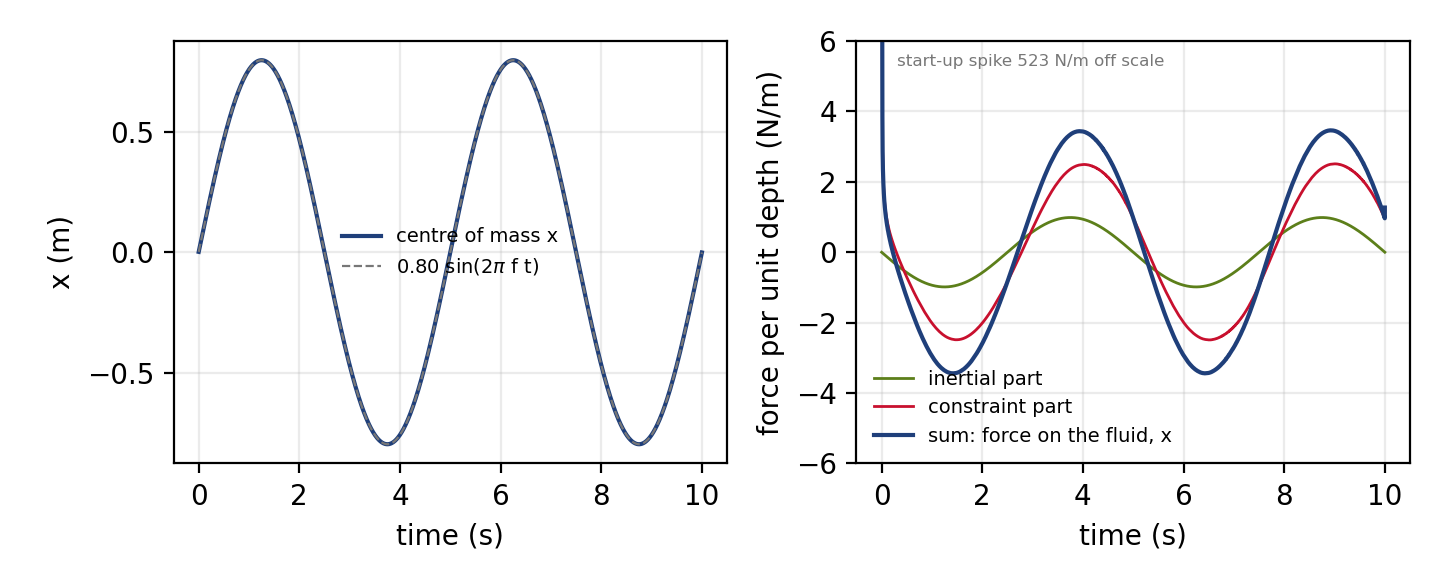
\includegraphics[width=\textwidth]{ch14-oscillating-cylinder}
\end{column}
\begin{column}{0.4\textwidth}
\scriptsize Left: the centre of mass from \code{Cylinder\_COM\_coordinates\_struct\_no\_0} against the integral of the prescribed velocity, $0.80\sin 2\pi f t$. Right: the two parts of the force on the fluid from \code{Cylinder\_Drag\_force\_struct\_no\_0}, and their sum.
\vspace{1mm}

\scriptsize Measured: the centre of mass reaches $0.7958$ m at $t = 1.25$ s, which is $U_\infty/2\pi f$, and never departs from $0.80\sin 2\pi f t$ by more than $10^{-6}$ m. The force: next slide.
\vspace{1mm}

\end{column}
\end{columns}
\sourcecredit{ConstraintIB/01 with IBAMR 0.19.0, 8 ranks; \code{tools/ch14\_figures.py} reads the method's text outputs.}
\end{frame}

% 16b
\begin{frame}{ConstraintIB/01: reading the force}
\label{fr:ex01c}
\footnotesize
\begin{itemize}
  \item In the second period the force on the fluid swings between $-3.44$ and $+3.46$ N/m. Its Fourier component in phase with the acceleration is $3.36$ N/m; the inviscid estimate for a disc of the fluid's density, the displaced fluid plus an equal added mass, is $2\rho\pi R^2 a_{\max} = 1.97$ N/m, so the fluid at $\mathrm{Re} = 100$ and $\mathrm{KC} = 5$ resists the acceleration $1.7$ times more than ideal flow would: the wake the disc runs back into is part of what it must accelerate.
  \item The component in phase with the velocity is $0.91$ N/m, a drag coefficient $2F/\rho U_\infty^2 D$ of $1.8$; the drag on the cylinder is minus the force on the fluid.
  \item The first period's force has the same shape except for its first step, a spike of $523$ N/m that the plot's scale leaves out: the velocity jumps from $0$ to $U_\infty$ at $t = 0$ and the method supplies that impulse in one step. A ramp (\code{U\_infinity} times $\min(t/t_r, 1)$ in the kinematics class) removes it; the upstream example does not bother, since it runs $26$ periods.
  \item The two parts the file keeps separate (slide \ref{fr:files}): the inertial part follows the acceleration of the body's own fluid, the constraint part is everything the fluid outside did not already provide; the paper's section 7.1.4 is about why a body with a changing velocity needs both.
\end{itemize}
\vspace{1mm}

\scriptsize The lecture's picture (slide 4) was VisIt's vorticity at $t = 72$ s with the disc's points over it: a pair of vortices either side of the disc, blue and red, left behind at each reversal. Chapter 26's recipe makes it from \code{viz\_cylinder2d}.
\end{frame}

% 17
\begin{frame}[fragile]{ConstraintIB/02: the impulsively started cylinder}
\label{fr:ex02}
\begin{columns}[T,onlytextwidth]
\begin{column}{0.46\textwidth}
\footnotesize ``This example appears in the paper in section 7.2.2. `We take the case of impulsively started cylinder in a quiescent flow to demonstrate the momentum-conservation properties of our method. A cylinder of diameter $D = 1$ m is placed at the center of a periodic domain of size 32 m x 16 m at time $t = 0$. An impulse of the form $I(t) = 400\exp(-400t)$ N/m$^3$ is applied in the $x$ direction within the body, at its initial position, thereby impulsively starting its motion.' This is an example of rigid body motion.'' (2020, slide 13)
\vspace{1mm}

\footnotesize ``Cylinder2d.vertex. As before, contains a list of x,y coordinates of the vertices. Spacing is dx=ds.'' (slide 14): $795$ points $1/32$ m apart, three levels, from the same generator as 01 with $1024$ cells per $32$ m.
\end{column}
\begin{column}{0.52\textwidth}
\begin{lstlisting}[style=inputtiny]
// input2d (ConstraintIB/02): the impulse is a body force on the fluid
ForcingFunction {
    XCOM = 0.0
    YCOM = 0.0
    RADIUS = R
    F      = RHO/DT_MAX
    function_0 = "(X0 - XCOM)^2 + (X1-YCOM)^2  < RADIUS^2
                     ? 400*exp(-400*t) : 0"        // one line in the file
    function_1 = "0.0"
}
ConstraintIBKinematics {
     Cylinder2d {
     structure_names                  = "cylinder2d"
     structure_levels                 =  MAX_LEVELS - 1
     calculate_translational_momentum = 1,1,0
     calculate_rotational_momentum    = 0,0,1
     lag_position_update_method       = "CONSTRAINT_VELOCITY"
     tagged_pt_identifier             = MAX_LEVELS - 1, 0
     kinematics_velocity_function_0   = "0.0"
     kinematics_velocity_function_1   = "0.0"
    }
}
\end{lstlisting}
\end{column}
\end{columns}
\end{frame}

% 17b
\begin{frame}{ConstraintIB/02 (2): what to notice, and slide 15 corrected}
\label{fr:ex02c}
\footnotesize
\begin{itemize}
  \item the force lives in the input: a muParser expression with a ternary, non-zero inside the disc only, registered by the \code{ForcingFunction} hook of \code{main.cpp} (chapter 7); its time integral is $1$ N s/m$^3$, so the impulse is the disc's area, $\pi/4$ per metre of depth; \code{F = RHO/DT\_MAX} is defined and unused;
  \item the body is free in $x$, $y$ and rotation; its kinematics velocity is zero (``0.0'' for both components; a missing one gives a warning and zero);
  \item \code{needs\_divfree\_projection = TRUE} and \code{output\_eulerian\_mom = TRUE} in the method's block: the correction is projected, and the fluid's total momentum is written to \code{CylinderDiv\_EULERIAN\_MOMENTUM.TXT};
  \item \code{Re = 200} sets \code{MU = 2.0*R/Re}; the run is $4$ s instead of ``10000'' (run until stopped), two and a half minutes on 4 ranks.
\end{itemize}
\vspace{1mm}

\scriptsize \al{Slide 15 corrected.} ``RigidBodyKinematics.cpp. This file is used to determine the rigid body motion of the cylinder. An applied force that decays over time is applied to the cylinder. The center of mass is calculated as well as the translational and rotational momentum. This is used to update the position of the immersed boundary. Remember to include RigidBodyKinematics.h'' The class does none of the middle three things: it evaluates the two \code{kinematics\_velocity\_function} expressions, nothing more; the force is the input's \code{ForcingFunction}, applied by the fluid solver, and the centre of mass and momenta are the method's, by the \code{calculate\_*} flags. The header must indeed be included. Slide 17's \code{function\_1 = "0.0“} ended in a curly quote, which the input parser rejects; the file has straight quotes (chapter 16).
\end{frame}

% 18
\begin{frame}{ConstraintIB/02: what it does}
\label{fr:ex02b}
\begin{columns}[T,onlytextwidth]
\begin{column}{0.58\textwidth}
\centering
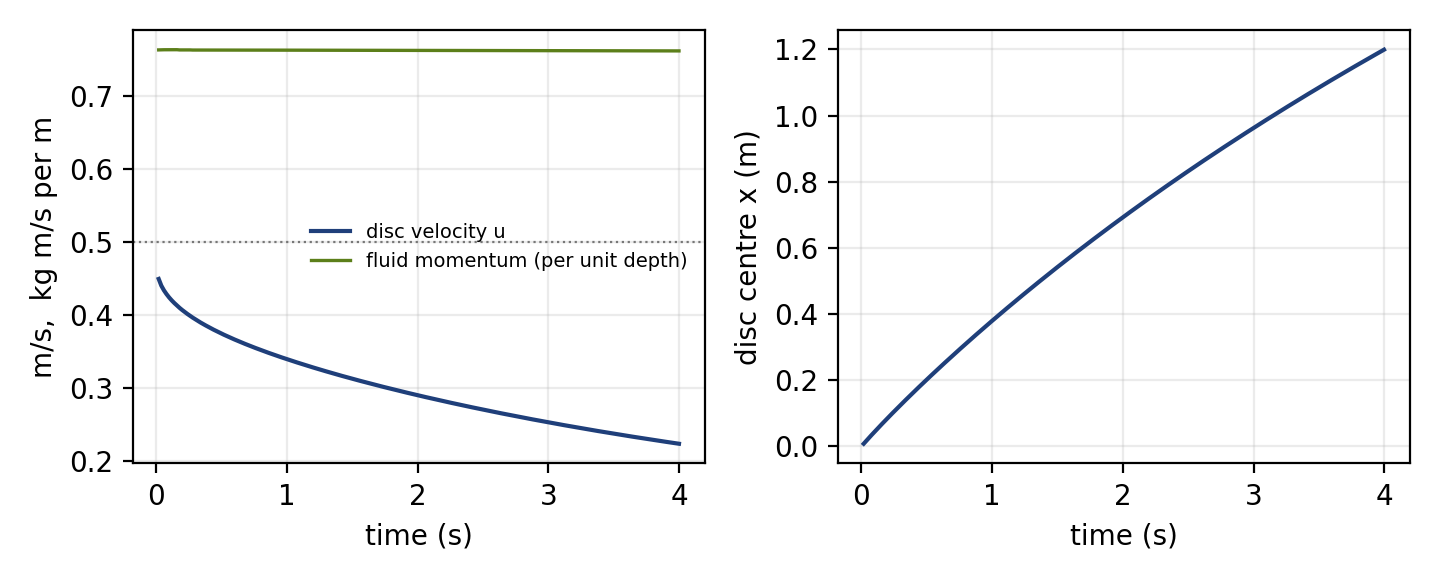
\includegraphics[width=\textwidth]{ch14-impulsive-cylinder}
\end{column}
\begin{column}{0.4\textwidth}
\scriptsize Left: the disc's velocity (\code{CylinderDiv\_Trans\_vel\_struct\_no\_0}) and the fluid's total momentum (\code{CylinderDiv\_EULERIAN\_MOMENTUM.TXT}). Right: the disc's position.
\vspace{1mm}

\scriptsize Measured: the disc's velocity peaks at $0.449$ m/s at $t = 0.02$ s, when the impulse is spent, against $0.5$ for an ideal disc of the fluid's density taking half the impulse; it is $0.42$ at $0.1$ s, $0.34$ at $1$ s and $0.22$ at $4$ s, by which time the disc has moved $1.20$ m. The momentum: next slide.
\vspace{1mm}

\end{column}
\end{columns}
\sourcecredit{ConstraintIB/02 with IBAMR 0.19.0, 4 ranks; \code{tools/ch14\_figures.py}.}
\end{frame}

% 18b
\begin{frame}{ConstraintIB/02: reading the momentum}
\label{fr:ex02d}
\footnotesize
\begin{itemize}
  \item The fluid's total momentum (\code{CylinderDiv\_EULERIAN\_MOMENTUM.TXT}) is $0.764$ at $0.1$ s and $0.762$ at $4$ s: conserved to $0.2$ per cent over $2{,}000$ steps. The value is what the impulse delivered: $795$ forcing cells of $1/32$ m give $0.776$ (the disc's area is $0.785$; the ternary counts cell centres).
  \item Why the disc's velocity is half of the impulse per unit mass: the impulse is delivered to the fluid in the disc region; to move, the disc must also move the fluid around it, and for a cylinder the added mass equals the displaced mass, so a body of the fluid's density takes half the momentum and leaves half in the fluid. The measured $0.449$ against $0.5$ is the viscous boundary layer and the grid's rendering of the disc's edge.
  \item The total stays put because the constraint force only moves momentum between body and fluid, it makes none, and a periodic box has no walls to absorb it. Then viscosity slows the disc at $\mathrm{Re} = 200$: $0.42$ at $0.1$ s, $0.34$ at $1$ s, $0.22$ at $4$ s.
  \item The angular velocity (\code{CylinderDiv\_Rot\_vel\_struct\_no\_0}) stays below $0.006$ s$^{-1}$: nothing in a symmetric problem turns the disc, and the method does not invent a torque.
\end{itemize}
\end{frame}

% 19
\begin{frame}{ConstraintIB/03: the swimming eel, as the lecture introduced it}
\label{fr:ex03}
\footnotesize ``ConstraintIB -- eel2d. In this example, the body deforms in a prescribed manner but is propelled through the water due to rigid body motion. The center of mass is calculated at each time as well as the translational and rotational momentum. This is used to update the position.'' (2020, slide 19, with the VisIt picture of slide \ref{fr:ex03b})
\vspace{1mm}

\footnotesize ``eel2d\_straightswimmer. This is a MATLAB code that generates the vertices for the eel. Eel2d.vertex is the output file.'' (slide 20)
\vspace{1mm}

\footnotesize ``IBEELKinematics.cpp. The default just allows for straight swimming of the eel. The deformation of the body is prescribed. The propulsion is based on rigid body kinematics. There are other functions for chasing a target / food, swimming in a circle, etc. This makes the code a little harder to understand. \code{if (d\_bodyIsManeuvering)} -- eel is maneuvering (turned off now). In such cases, the maneuver axis is used to transform the body. Deformation velocity functions are read in from the input file. Center of mass is calculated at each time.'' (slide 21)
\vspace{1mm}

\footnotesize Slides 22 and 23 (``Input2d -- Constraint IB Method'', ``Input2d -- body shape equation'') were screenshots of the two input blocks, retyped on the next slide.
\end{frame}

% 19b
\begin{frame}[fragile]{ConstraintIB/03 (2): the input block}
\label{fr:ex03in}
\begin{lstlisting}[style=inputtiny]
// input2d (ConstraintIB/03): the eel's sub-block; the three long expressions are one line each in the file
eel2d {
     structure_names                  = "eel2d"
     structure_levels                 =  MAX_LEVELS - 1
     calculate_translational_momentum = 1,1,0
     calculate_rotational_momentum    = 0,0,1
     lag_position_update_method       = "CONSTRAINT_POSITION"
     tagged_pt_identifier             = MAX_LEVELS - 1, 0  // level, relative idx of lag point
     initial_angle_body_axis_0         = 0.0                     //default 0.0
     body_shape_equation               = "0.125* ( (X_0 + 0.03125)/1.03125 ) * sin( 2*PI*X_0 - (0.785/0.125)*T )"
     deformation_velocity_function_0   = "( -0.785* ( (X_0 + 0.03125)/1.03125 )
                                            *cos( 2*PI*X_0 - (0.785/0.125)*T ) )*N_0"
     deformation_velocity_function_1   = "( -0.785*  ( (X_0 + 0.03125)/1.03125 )
                                            *cos( 2*PI*X_0 - (0.785/0.125)*T ) )*N_1"
     body_is_maneuvering                 = FALSE       //default false. If FALSE then nothing below has any effect.
     maneuvering_axis_equation           = "sqrt(1.3^2 -(X_0 - 0.5)^2) - 1.2"     //"0.1*sin(PI*X_0)"
     maneuvering_axis_is_changing_shape  = TRUE  // should be true.
     food_location_in_domain_0         =  1.0
     food_location_in_domain_1         = -3.3
}
\end{lstlisting}
\footnotesize The shape in the body frame, $y = 0.125\,\frac{x + 0.03125}{1.03125}\sin(2\pi x - 6.28\,t)$ for $x$ from the nose ($0$) to the tail ($1$): one wavelength on the body, travelling tailward at one length per second, amplitude from $0.004$ at the nose to $0.125$ at the tail. The velocity functions are its time derivative, applied along the body normal (\code{N\_0}, \code{N\_1}; slide \ref{fr:keys2}). The amplitude and frequency appear in all three expressions and must be changed together.
\end{frame}

% 19c
\begin{frame}{ConstraintIB/03 (3): what to notice}
\label{fr:ex03c}
\footnotesize
\begin{itemize}
  \item \code{CONSTRAINT\_POSITION}: each step the class \emph{sets} the shape (\code{setShape}) and the method adds the rigid translation and rotation it computes, so the body never drifts from its prescribed form; with \code{CONSTRAINT\_VELOCITY} the integrated velocity would slowly deform it;
  \item the flags unlock $x$, $y$ and rotation: the eel yaws as well as swims, and the \code{Rot\_vel} file records it; the deformation's own momentum (the wave as written is not momentum-free) is measured each step and subtracted, so only the fluid can propel the eel;
  \item $2{,}932$ points filling the body, one finest cell apart, from \code{eel2d\_straightswimmer.m}: a rounded head $0.04$ wide and a linear taper to the tail; nose at $x = -0.5$, tail at $0.5$; the Python port writes the same file;
  \item $\mathrm{Re} = 5609$ on the tail's lateral speed $0.785$ (\code{MU = 0.785/Re}); an $8\times4$ m periodic box with six body lengths of room ahead; finest cells $1/256$ m (ten across the head); \code{DT\_MAX = 0.0001}, $10{,}000$ steps per beat;
  \item \code{main.cpp} also carries an \code{IBHydrodynamicForceEvaluator}: the force on the eel from a control volume (\code{InitHydroForceBox\_0}, $2 \times 1.4$ m) that moves with it, written to \code{Drag\_CV\_strct\_id\_0} and \code{Torque\_CV\_strct\_id\_0} (chapter 11's other way to a force; Nangia et al.\ 2017);
  \item two beats ($2$ s) instead of the upstream $10$ s, 12 minutes on 8 ranks; the upstream restart dumps every $150$ steps are switched off.
\end{itemize}
\end{frame}

% 20
\begin{frame}{ConstraintIB/03: what it does}
\label{fr:ex03b}
\begin{columns}[T,onlytextwidth]
\begin{column}{0.58\textwidth}
\centering
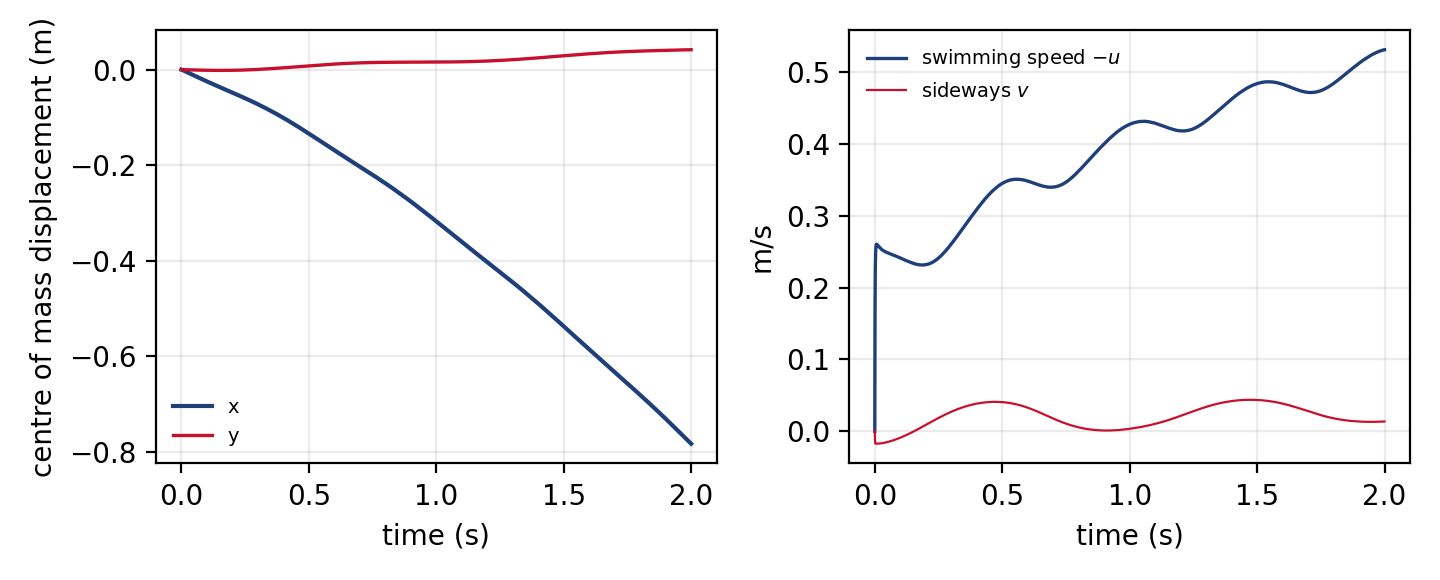
\includegraphics[width=\textwidth]{ch14-eel-swimming}
\end{column}
\begin{column}{0.4\textwidth}
\scriptsize Left: the centre of mass (\code{Eel2d\_COM\_coordinates\_struct\_no\_0}). Right: the swimming speed and the sideways velocity (\code{Eel2d\_Trans\_vel\_struct\_no\_0}).
\vspace{1mm}

\scriptsize The numbers: next slide.
\end{column}
\end{columns}
\sourcecredit{ConstraintIB/03 with IBAMR 0.19.0, 8 ranks; \code{tools/ch14\_figures.py}.}
\end{frame}

% 20b
\begin{frame}{ConstraintIB/03: reading the swim}
\label{fr:ex03d}
\footnotesize
Measured: the centre of mass moves $-0.32$ m in the first beat and $-0.47$ m in the second, $-0.78$ m in all with $0.04$ m sideways: the eel is still accelerating, from $0.32$ to $0.47$ lengths per beat (the speed jumps to $0.26$ m/s in the first step, because the wave starts at full amplitude at $t = 0$, and climbs from there with a dip at every half beat). The lecture's picture at $t = 1$ s, the body between $x = -0.8$ and $0.25$, is the first beat's $0.32$. The yaw rate reaches $0.47$ s$^{-1}$; the deformation's centre-of-mass velocity, which the method removes each step, reaches $0.07$ m/s.
\vspace{2mm}

\footnotesize What to take from it: a free swimmer in the constraint method moves only by what its prescribed wave does to the fluid, so the speed is an outcome, not an input; two beats are not enough for a steady speed (the upstream $10$ s run is), and the eel yaws a little as it goes, which \code{calculate\_rotational\_momentum = 0,0,0} would forbid.
\vspace{2mm}

\scriptsize The lecture's picture (slide 19, VisIt, $t = 1$ s, cycle 10000): the body between $x = -0.8$ and $0.25$, having started between $-0.5$ and $0.5$, with the boundary layers of opposite sign along its two sides and a vortex pair shed from the tail trailing behind at $x \approx 0.4$ to $0.5$. The wave travels tailward, so the eel swims toward $-x$. Chapter 26 reproduces it from \code{viz\_eel2d\_Str}.
\end{frame}

% 21
\begin{frame}[fragile]{Reading the outputs}
\label{fr:read}
\begin{columns}[T,onlytextwidth]
\begin{column}{0.5\textwidth}
\begin{lstlisting}[style=pythontiny]
# Python: the disc's velocity after the impulse (ConstraintIB/02)
import numpy as np
v = np.loadtxt("Cylinder_Dump/CylinderDiv_Trans_vel_struct_no_0")
t, u = v[:, 0], v[:, 1]            # time, rigid velocity x
print(u.max(), t[u.argmax()])      # the peak and when
p = np.loadtxt("Cylinder_Dump/CylinderDiv_EULERIAN_MOMENTUM.TXT")
print(p[-1, 1])                    # the fluid's x momentum at the end
\end{lstlisting}
\begin{lstlisting}[style=matlabtiny]
% MATLAB/Octave: the force on the oscillating cylinder (ConstraintIB/01)
d = load('Dump--Cylinder/Cylinder_Drag_force_struct_no_0');
t = d(:,1); F = d(:,2) + d(:,5);   % inertial + constraint, x
plot(t, -F); xlabel('t (s)'); ylabel('drag on the cylinder (N/m)');
\end{lstlisting}
\end{column}
\begin{column}{0.48\textwidth}
\footnotesize The files are plain tab-separated numbers with no header, so \code{np.loadtxt} and \code{load} read them whole; the column meanings are on slide \ref{fr:files}. Two cautions:
\begin{itemize}
  \item a file is written every \code{output\_interval} steps, and the position file is written at the \emph{start} of the step (\code{d\_FuRMoRP\_current\_time}) while the velocity and force files carry the end (\code{new\_time}): their first lines differ by one step;
  \item a quantity that was switched off leaves an empty file, which \code{loadtxt} refuses; check \code{PrintOutput} rather than the folder.
\end{itemize}
\scriptsize \code{tools/ch14\_figures.py} in the tutorial repository does this for the three examples and prints the numbers quoted on their slides; it is twenty lines per example.
\end{column}
\end{columns}
\end{frame}

% 22
\begin{frame}[fragile]{Running the three on Puma, and what they cost}
\label{fr:puma}
\begin{lstlisting}[style=shell]
# from the example folder, after enable.sh (chapter 1)
cmake -S . -B build -DCMAKE_BUILD_TYPE=Release
cmake --build build -j 4
sbatch job.slurm          # 4 tasks; edit --account; the outputs: viz_*/ for VisIt, the text files in Dump--Cylinder/, Cylinder_Dump/ or Eel2dStr/
\end{lstlisting}
\begin{center}
\scriptsize
\begin{tabular}{@{}llllll@{}}
\toprule
example & steps & finest cells & levels & ranks & wall time\\
\midrule
01 oscillating cylinder, two periods & $6{,}667$ & $1/128$ m & 4 & 8 & 11 min\\
02 impulsively started cylinder, $4$ s & $2{,}000$ & $1/32$ m & 3 & 4 & 2.5 min\\
03 eel, two beats & $20{,}000$ & $1/256$ m & 3 & 8 & 12 min\\
\bottomrule
\end{tabular}
\end{center}
\footnotesize Each folder's \code{job.slurm} is chapter 1's with the job name and a time limit chosen from these runs; \code{CMakeLists.txt} lists the program and the kinematics class. The times are from a desktop PC under WSL (chapter 2), the three running at once with \code{mpirun --bind-to none}. The upstream lengths ($130$ s, ``10000'' s and $10$ s) are $13$, $2500$ and $5$ times longer: those are Puma jobs, and the reason for the lecture's warning about files.
\end{frame}

% 23
\begin{frame}{What can go wrong (1): the messages}
\label{fr:wrong}
\scriptsize
\setlength{\tabcolsep}{3pt}
\begin{tabular}{@{}L{0.34\textwidth}L{0.34\textwidth}L{0.26\textwidth}@{}}
\toprule
what you see & why & fix\\
\midrule
\code{Structure cylinder2d does not} \code{exist on level 2} & \code{structure\_levels} in the kinematics block and \code{level\_number} in \code{IBStandardInitializer} disagree, or the name is misspelt & make the three names and the two levels agree\\
\code{Update methods supported are} \code{CONSTRAINT\_VELOCITY,} \code{CONSTRAINT\_POSITION AND} \code{CONSTRAINT\_EXPT\_POSITION} & \code{lag\_position\_update\_method} is anything else & use one of the three\\
\code{Could not tag Lagrangian point} \code{for this structure} & \code{tagged\_pt\_identifier}'s level is not one of the structure's & level first, then the relative index\\
\code{frequency of cylinder does not} \code{exist in the InputDatabase} & the subclass requires its keys & add \code{frequency}, \code{U\_infinity}\\
\code{Total levels > 1,} \code{OscillatingCylinder should be} \code{places on only one level} & the structure spans levels & put it on one level\\
\code{no function corresponding to key} \code{kinematics\_velocity\_function\_1} & a warning, not a stop: the component is set to \code{"0.0"} & add the key if you meant something else\\
\bottomrule
\end{tabular}
\vspace{1mm}

\scriptsize The messages are the sources' (\code{ConstraintIBKinematics.cpp}, \code{OscillatingCylinderKinematics.cpp}, \code{RigidBodyKinematics.cpp}); ``places'' is the source's spelling. Chapter 16 has the general ones (CFL, parse errors, Puma limits).
\end{frame}

% 23b
\begin{frame}{What can go wrong (2): the silent ones}
\label{fr:wrong2}
\scriptsize
\setlength{\tabcolsep}{3pt}
\begin{tabular}{@{}L{0.3\textwidth}L{0.38\textwidth}L{0.26\textwidth}@{}}
\toprule
what you see & why & fix\\
\midrule
nothing is printed, or the wrong things & \code{PrintOutput} must be \emph{inside} \code{ConstraintIBMethod}; unknown keys there are ignored without a word (the 2020 slide 10) & the list of slide \ref{fr:method}\\
a parse error at a quote & a curly quote pasted from a slide (\code{"0.0“}) & straight quotes (chapter 16)\\
the disk fills & restart every 150 steps, viz every 40, 100,000 steps & raise the intervals; the examples' READMEs\\
the body drifts from its shape & \code{CONSTRAINT\_VELOCITY} with a deformation integrates errors & \code{CONSTRAINT\_POSITION}, as the eel\\
the body does not move although it is free & the deformation carries momentum, which the method removes; or the flags are \code{0,0,0} & check \code{calculate\_*}; give the fluid a push (a body force) or a wave that pushes fluid\\
a heavier body falls no faster & \code{rho\_solid} does not add inertia & a gravity body force in the body's region (the falling sphere), or chapter 13\\
\bottomrule
\end{tabular}
\end{frame}

% 24
\begin{frame}{Constraint IB among IBAMR's rigid-body tools}
\label{fr:tools}
\footnotesize
\begin{itemize}
  \item \al{\code{ConstraintIBMethod}} (this chapter): a region of fluid made to move as a rigid or prescribed-deformation body by a velocity correction after each solve; free motion from the momentum in the body; 2D and 3D; \code{examples/ConstraintIB}.
  \item \al{\code{CIBMethod}} (chapter 15 tours its \code{examples/CIB}): the constraint written as a saddle-point problem with a mobility solver, for Stokes and low-Reynolds-number suspensions of many rigid bodies; the lecture: ``Some examples are also similar to the CIB ones.''
  \item \al{\code{IBFEDirectForcingKinematics}}: the same idea for an IBFE mesh (Part IV), with the body a finite-element volume.
  \item \al{\code{BrinkmanPenalizationRigidBodyDynamics}}: a level-set body made rigid by a Brinkman penalty term in the momentum equation, with the body's dynamics integrated; the level-set examples.
  \item \al{\code{PenaltyIBMethod}} (chapter 13): mass on a copy of a point; not rigid, but heavy.
  \item \al{Target points} (chapter 9a): a rigid body of the standard method, held by tethers; the simplest, and the stiffest.
\end{itemize}
\begin{punchbox}
\footnotesize Prescribed motion of a rigid shape through a fluid, or a body whose deformation you know: constraint IB. A body whose deformation the fluid decides: IBFE. Many rigid particles in Stokes flow: CIB.
\end{punchbox}
\end{frame}

% 25
\begin{frame}{Homework}
\label{fr:hw}
\footnotesize
\begin{enumerate}
  \item ConstraintIB/01: do the lecture's exercise (slide 7, ``Alter the kinematics to make the cylinder go up and down''): write \code{[0][1][k]} instead of \code{[0][0][k]} and compare the $y$ force file with the $x$ one of the shipped run. Then tow it (\code{U\_infinity = 0}, \code{prescribed\_trans\_velocity = 1}) and read the drag coefficient $C_D = 2F/(\rho U^2 D)$ from the force file after it settles (chapter 11).
  \item ConstraintIB/02: push the disc off centre (\code{XCOM = 0.2}) so that the impulse has a moment; read the angular velocity file. Then repeat with \code{needs\_divfree\_projection = FALSE} and say what changed in the momentum file.
  \item ConstraintIB/03: halve the amplitude ($0.125 \to 0.0625$ in all three expressions) and run two beats; compare the swimming speed. Then switch \code{body\_is\_maneuvering = TRUE} and watch where the eel goes.
  \item Write a kinematics class of your own: a disc that rolls (prescribed angular velocity, zero translation) by filling \code{d\_current\_kinematics\_vel} with $\boldsymbol{\Omega}\times\mathbf{R}$ about the centre of mass, which \code{setKinematicsVelocity} receives. Start from \code{OscillatingCylinderKinematics}.
  \item Add a second structure: two discs, each with its own kinematics object and sub-block, \code{num\_structures = 2}; the force files get a \code{\_struct\_no\_1}.
\end{enumerate}
\end{frame}

% 26
\begin{frame}{Rules of thumb}
\label{fr:thumb}
\small
\begin{itemize}
  \item \code{ConstraintIBMethod} + one kinematics object per structure + two input blocks; register, then \code{initializeHierarchyOperatorsandData()}.
  \item A kinematics class sets a velocity per point per component; the method adds the rigid motion for the free components (\code{calculate\_*} flags) and removes the deformation's own momentum.
  \item One level per structure; names and levels must agree in three places.
  \item \code{PrintOutput} inside the method's block; the keys of slide \ref{fr:method}; the files of slide \ref{fr:files}; \code{np.loadtxt} reads them.
  \item Body density is the fluid's; a heavier body gets a body force in its region.
  \item Prescribed deformation: \code{CONSTRAINT\_POSITION}. Rigid: \code{CONSTRAINT\_VELOCITY}.
  \item Fill the body with points one finest cell apart (\code{Cylinder2d.m}: ``ds = dx'').
  \item Shorten the upstream runs and dump intervals before the first run.
\end{itemize}
\end{frame}

% 27
\begin{frame}{Summary}
\label{fr:summary}
\footnotesize
\begin{enumerate}
  \item The constraint IB method solves the fluid everywhere and then corrects the velocity inside a body to the rigid or prescribed-deformation motion the body should have; the correction's cost is the hydrodynamic force, written every step.
  \item A program needs \code{ConstraintIBMethod}, a \code{ConstraintIBKinematics} subclass with four functions, and two input blocks: the structure's (names, levels, the free-component flags, the update method, a tagged point, the class's own keys) and the method's with \code{PrintOutput}.
  \item Locked flags give prescribed motion (01); free flags with zero kinematics give a rigid body moved by the fluid's momentum (02); free flags with a deformation give a swimmer (03).
  \item The outputs are plain text: drag, torque, power, velocities, centre of mass, moments of inertia, the fluid's momentum; four lines of Python or MATLAB read them.
  \item The three examples run in minutes to an hour on a desktop PC (WSL) and reproduce the lecture's pictures; the 2020 slides' three slips (a key that does not exist, a file name, what \code{RigidBodyKinematics} does) are corrected here.
\end{enumerate}
\begin{homebox}
\footnotesize Chapter 15 tours the rest of IBAMR's examples, ConstraintIB's nine among them; chapter 16 collects what can go wrong.
\end{homebox}
\end{frame}

% 28
\begin{frame}{What changed since the older course notes}
\label{fr:changed}
\footnotesize
\begin{itemize}
  \item The 2020 lecture showed files; this chapter says what the method does with them (slides \ref{fr:what}, \ref{fr:step}, \ref{fr:free}), from the source, and runs the three examples with measured results.
  \item The input keys are the verified list: slide 10's \code{output\_drag\_kinetic\_energy} does not exist and its block was never read; slide 8's ``coarsest grid spacing'' is a cell count; slide 5's \code{2dcylinder.vertex} is \code{cylinder2d.vertex}; slide 15's account of \code{RigidBodyKinematics.cpp} is corrected; slide 17's curly quote is straightened.
  \item The examples are shipped with the tutorial's CMake build, shortened runs, Python ports of the generators checked against Octave and against the upstream files, READMEs with the output formats, and a figure script.
  \item Lecture 6's six slides on the ConstraintIB set are merged in (the table of slide \ref{fr:nine}), so the chapter stands alone; the CIB set is left to chapter 15.
\end{itemize}
\end{frame}

% 29
\begin{frame}{Recordings (listed, not incorporated)}
\label{fr:videos}
\small The 2020 Zoom recordings of IBAMR Lecture 7 (\emph{Constraint IB}, two files, with and without sound, 2020-09-09) and of Lecture 6 (\emph{Boyce's examples}) exist in the course's Drive folder and are listed in the front matter's video list (chapter 0.1). They were taught from the slides quoted here, and nothing in them is reproduced in this chapter.
\end{frame}

% 30
\begin{frame}{References}
\label{fr:refs}
\scriptsize
\begin{itemize}
  \item A. P. S. Bhalla, R. Bale, B. E. Griffith and N. A. Patankar, \emph{A unified mathematical framework and an adaptive numerical method for fluid--structure interaction with rigid, deforming, and elastic bodies}, Journal of Computational Physics 250 (2013) 446--476.
  \item N. Nangia, H. Johansen, N. A. Patankar and A. P. S. Bhalla, \emph{A moving control volume approach to computing hydrodynamic forces and torques on immersed bodies}, Journal of Computational Physics 347 (2017) 437--462 (the force evaluator of ConstraintIB/03).
  \item IBAMR 0.19.0: \code{include/ibamr/ConstraintIBMethod.h}, \code{src/IB/ConstraintIBMethod.cpp}, \code{include/ibamr/ConstraintIBKinematics.h}, \code{src/IB/ConstraintIBKinematics.cpp}, \code{examples/ConstraintIB/} (nine examples). \url{https://github.com/IBAMR/IBAMR}
  \item The examples of this series: ConstraintIB/01 oscillating cylinder, 02 impulsively started cylinder, 03 swimming eel (each with \code{main.cpp}, a kinematics class, \code{input2d}, a vertex file and its MATLAB and Python generators, \code{CMakeLists.txt}, \code{job.slurm}, README); \code{tools/ch14\_figures.py}.
  \item Sources: \emph{IBAMR Lecture 7: Looking at ConstraintIB examples of prescribed and rigid body motion} (2020, 23 slides) and \emph{IBAMR Lecture 6: What do Boyce's examples do} (2020), slides 17--24.
\end{itemize}
\end{frame}

\end{document}
